\documentclass[a4paper]{article}
\usepackage[utf8x]{inputenc}
\usepackage[danish]{babel}
\usepackage{utopia}
\usepackage{graphicx}
\usepackage{listings}
\usepackage{graphicx}
\usepackage{cmap}

\title{Heaps - ADS}
\author{Edi Begovic | Høgni Jacobsen | Gergö Koncz}
\date{\today}

\def\arraystretch{1.5}
\def\headline#1{\hbox to \hsize{\hrulefill\quad\lower.3em\hbox{#1}\quad\hrulefill}}

\begin{document} 
\maketitle

\ \\
\noindent
The pseudo-code will reference the queue on which the function is called as \textit{q}.
\ \\
\section*{Question 1}
Assuming we wish to draw the resulting binary tree of a max heap:
\ \\
\begin{center}
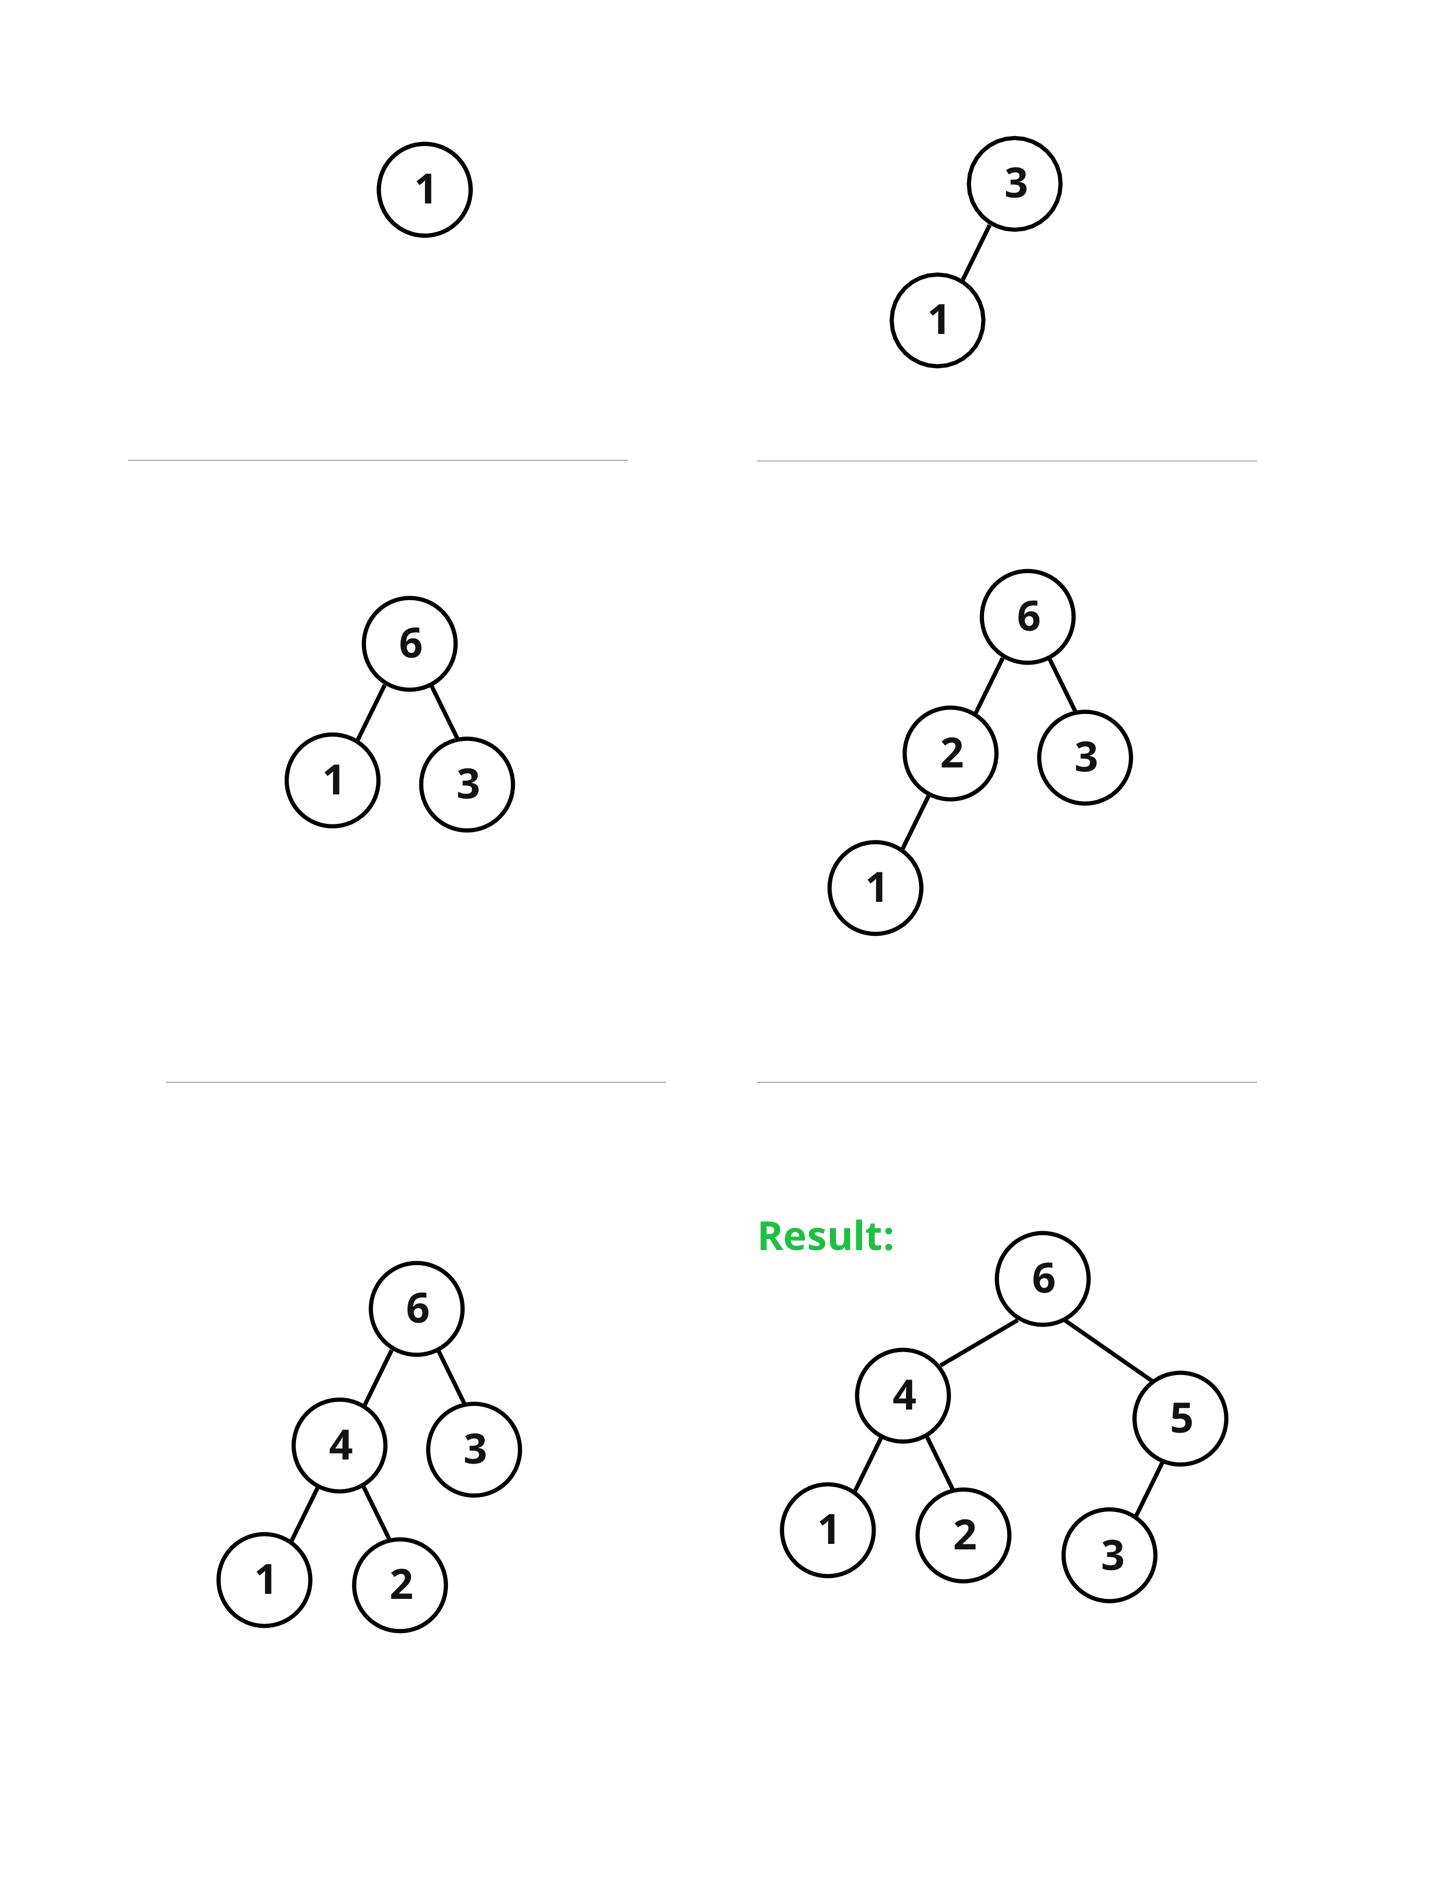
\includegraphics[scale=0.16]{figure1.png}
\end{center}

\noindent
This results in the following array representation: 
$[6, 4, 5, 1, 2, 3]$


\ \\
\section*{Question 2}
\headline{a} \ \\

\noindent
Assuming the 'first' implies the pointer to the first element in the list 
(\textit{that is}, that last added item (p. 148)), answer a is correct.
\ \\

\begin{center}
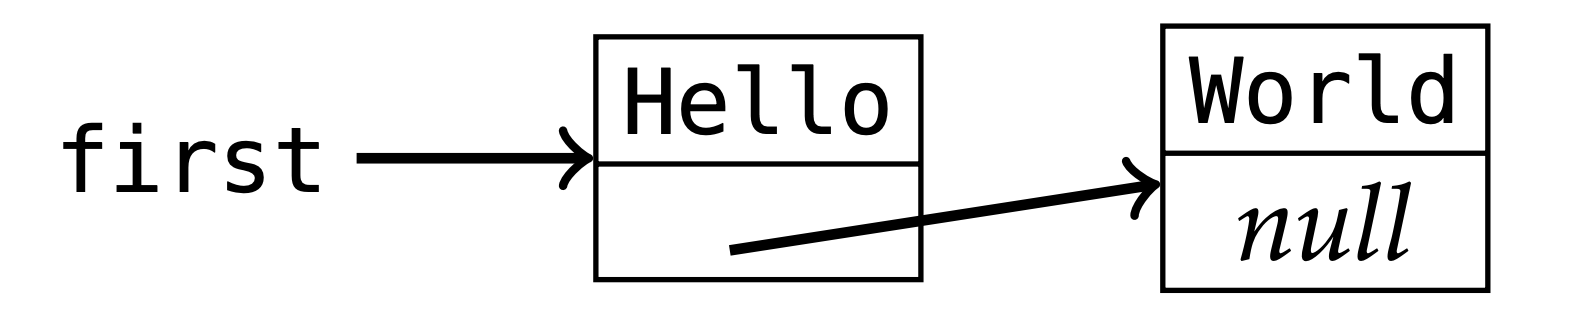
\includegraphics[scale=0.22]{figure2.png}
\end{center}

\end{document}